%!TEX root = ../summary.tex

\section{Introduction}
This lecture is about understanding how to build complex (software) systems, which trade-offs there are between quality and the architecture and how to efficiently deliver the developed software to the stakeholders.
For that, different modeling techniques, system analysis and design with quality trade-offs, patterns, guidelines and best-practices are taught and tools for system configuration, integration and deployment are explained.

The lecture is separated into 4 chapters:
\begin{enumerate}
    \item Context of Software Engineering
        \subitem {\small Introduction, characteristics of software systems in different domains, case studies and factors affecting the design of a software system}
    \item From (quality) requirements to system design
        \subitem {\small Software architecture, libraries and frameworks, antipatterns, model-driven engineering, software product line engineering, safety and security, testability}
    \item Software architectures and their trade-offs
        \subitem {\small Distributed systems and middleware, database-, message-, object-, component- and service-oriented architectures}
    \item From source code to physical deployment
        \subitem {\small Historical perspective, version control, continuous integration and deployment, virtual machines and containers, software architectures for the cloud}
\end{enumerate}

\subsection{Characteristics of Software Systems}
Software eningeering can be separated into the technical \& management and the application domain.
The technical \& management domain contain the software system with limiting factors.
First, there are different targets defining those borders: Beside the technical infrastructure which is defining the system's size, cost, quality, time and the functionality target are set limits.
Those factors again are influenced by the process (high control) used to develop the system and the constraints (limited control: money, stakeholders, environmental influences, ...) limiting the resources available during development of the system.

The application domain is influencing the functionality target (e.g. needed functionality, available inputs and outputs, ...) and the constrains (money, management, ...) in the technical \& management domain.

The application domain can be divided into 
\begin{itemize}[topsep=5pt, itemsep=0pt]
    \item \textbf{Embedded} systems \textit{electronic devices, transportation, intelligent homes, ...}
    \item \textbf{Information} systems \textit{logistics, marketing tools, management tools, ...}
    \item \textbf{Cyberphysical} systems (connects embedded and information system) \textit{networks, reading sensors and putting out information, ...}
    \item (\textbf{Scientific software} systems \textit{not covered})
\end{itemize}



\subsection{Definition: Software Engineering}
\begin{chapquote}{"Perspectives on software engineering." Zelkowitz. (1978)}
    Study of the principles and methodologies for developing and maintaining software systems.
\end{chapquote}
\begin{chapquote}{"Software engineering: methods and management." Pfleeger. (1990)}
    Methods and techniques to develop and maintain quality software to solve
    problems.
\end{chapquote}
\begin{chapquote}{"Software engineering." Sommerville. (2010)}
    Software engineering is an engineering discipline which is concerned with all
    aspects of software production.
\end{chapquote}

Software Engineering is a collection of \textbf{techniques}, \textbf{methodologies} and \textbf{tools} that help with the production of a \textbf{\textit{high quality}} software system with a \textbf{\textit{given budget}} before a \textbf{\textit{given deadline}} while \textbf{\textit{change occurs}}.
It is essentially a problem solving activity for which first the problem is analyzed and broken down into pieces to understand the nature of the problem and later is synthesized into a large structure using \textbf{techniques}, \textbf{methodologies} and \textbf{tools}.

\begin{itemize}
    \item \textbf{Techniques} Formal procedures for producing results using some well-defined notation
    \item \textbf{Methodologies} Collection of techniques applied across software development and unified by a philosophical approach
    \item \textbf{Tools}
        \begin{itemize}[topsep=-5pt, itemsep=0pt]
            \item Instruments or automated systems to accomplish a technique
            \item Integrated Development Environment (IDE)
            \item Computer Aided Software Engineering (CASE)
        \end{itemize}
\end{itemize}

\begin{figure}[h]
    \centering
    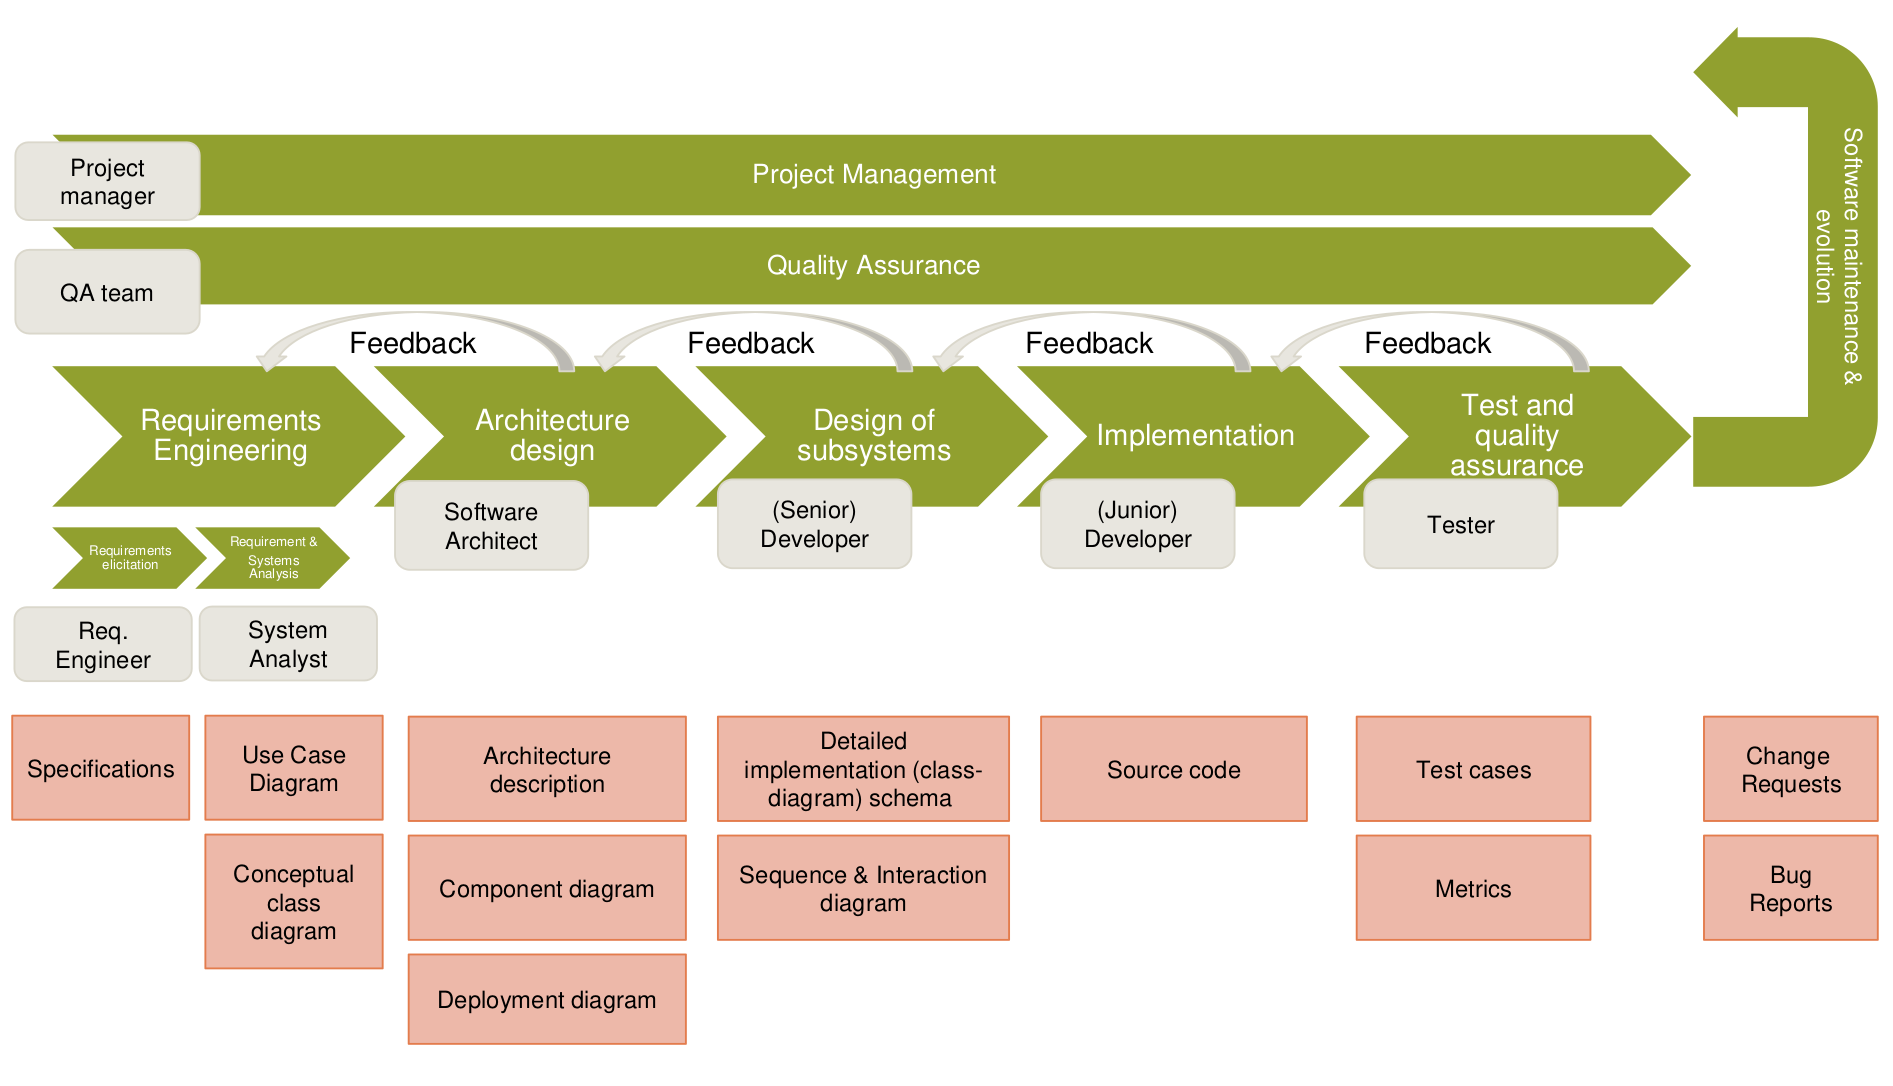
\includegraphics[width=\linewidth]{images/se_activities_roles_artifacts.png}
    \caption{Software Engineering Activities, Roles and Artifacts}\label{fig:se_activities_roles_artifacts}
\end{figure}

\subsubsection{The Process Model}
A process model describes the systematic, engineering-based, and quantifiable approach to solve a particular class of repeatable problems.
It is an abstract representation of the software process.

Some examples are:
\begin{itemize}
    \item Waterfall model \textit{\textbf{phase oriented}, classical/conventional model, inflexible (\textbf{sequential} procedure enforced), risky (errors found late and expensive)}
    \item V-Model \textit{Iterative model, \textbf{phase oriented, multiple pass}, loosely based on Waterfall, project definition then project test and integration}
    \item Unified Process \textit{Incremental model, development in expansion stages, 4 phases:Inception, Elaboration, Construction, Transition}
\end{itemize}

% TODO maybe more about unified process?

\paragraph{Agile development}
Focus on software to solve customer's problem. Less buerocratic approach. Example: Scrum (daily and stand up meetings, sprints (solving tasks from backlog))
\begin{itemize}
    \item \textbf{Individuals and interactions} over processes and tools
    \item \textbf{Working software} over comprehensive documentation
    \item \textbf{Customer collaboration} over contract negotiation
    \item \textbf{Responding to change} over following a plan
\end{itemize}

\subsubsection{Artifacts in Software Engineering}
The following lists artifacts generated during different stages of the software development process.
\paragraph{Requirements Engineering} Feasibility Report, System Models, User and System Requirements, Requirements Document
\paragraph{Software Design} System Architecture, Database Specification, Interface Specification, Component Specification
\paragraph{Testing} Acceptance Test Plan, System Integration Test Plan, Sub-System Integration Test Plan

\subsubsection{Software Quality}
\begin{chapquote}{loosely based on Balzert}
    Software quality refers to the entire characteristics of a software product that
    influence its ability to fulfill specified requirements and stakeholder expectations.
\end{chapquote}
\begin{chapquote}{"ISO 9000 - Quality management" http://www.iso.org/iso/iso\_9000}
    (Software) Quality is the degree to which a set of inherent characteristics fulfills requirements, meaning needs or expectations that are stated, generally implied or obligatory.
\end{chapquote}

Quality is a key factor for the product's success and customer's satisfaction.
In many cases quality demands are fixed (e.g. laws, contracts, ...).
Quality is tightly coupled with Non-functional requirements (NFR), but they are in general not the same.
In the lecture, quality is the sum of the process quality and the product quality (NFRs). It essentially is more than just NFRs.

Increased quality has trade-offs and can either support other quality aspects (e.g. maintainability vs. portability), or negatively influence them (security vs. efficiency).

To maximize the quality of a system, quality aspects and its interdependencies have to be assessed and balanced and prioritized in a way, where negative trade-offs are small.
Those trade-offs and prioritizations are highly situation and project dependent.

The quality of the developed product is influenced by the quality of the production process, but the correlation is complex (see \autoref{fig:se_process_vs_quality}), since software development is a creative, rather than a mechanical process.
Measuring the quality of software is difficult (e.g. measuring maintainability needs a long time).

\begin{figure}[h]
    \centering
    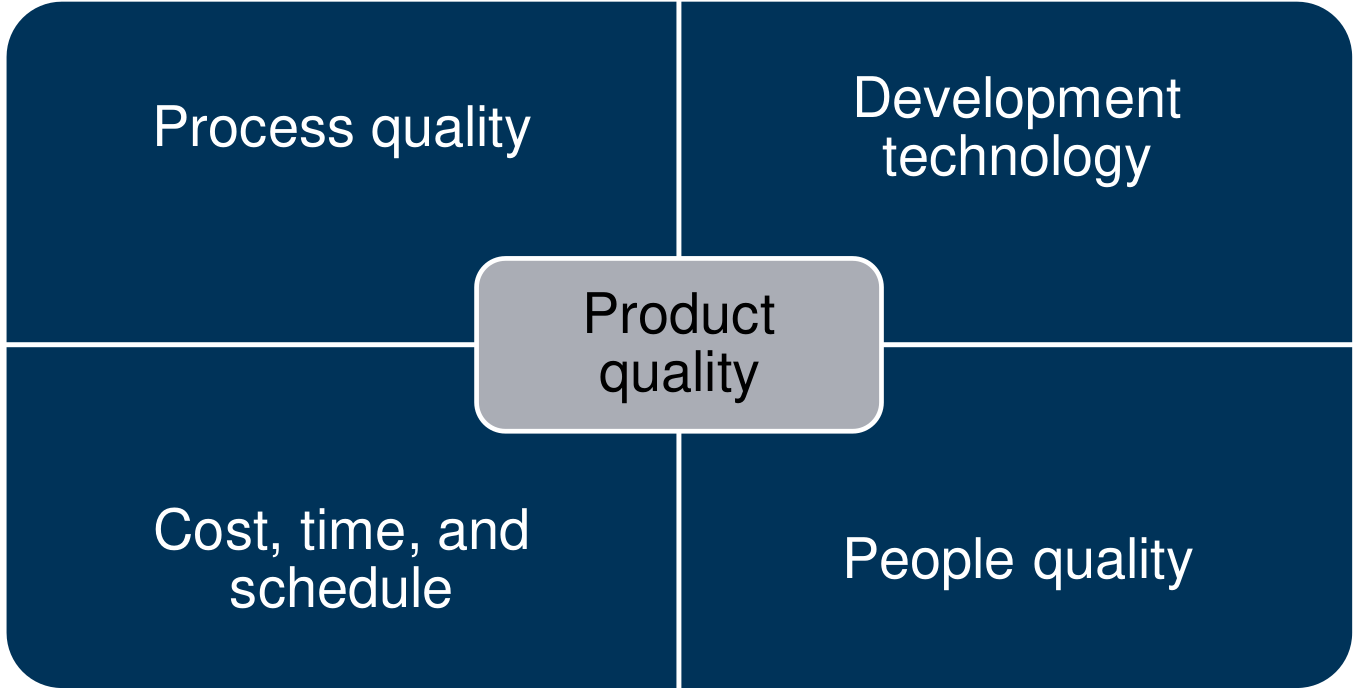
\includegraphics[width=0.5\linewidth]{images/process_vs_quality.png}
    \caption{Correlation between software process and quality}\label{fig:se_process_vs_quality}
\end{figure}

\paragraph{ISO 9000 and 9001}
This is an international set of standards for quality management and applicable to a range of organization branches.
If an organization is to be ISO 9001 conformant, it must document how its
processes relate to the nine core processes:\\

\begin{minipage}[t]{0.49\textwidth}
    \textbf{Product delivery process}
    \begin{itemize}[topsep=0pt, itemsep=0pt]
        \item Business acquisition
        \item Design and Development
        \item Test
        \item Production and delivery
        \item Service and support
    \end{itemize}
\end{minipage}
\begin{minipage}[t]{0.49\textwidth}
    \textbf{Supporting processes}
    \begin{itemize}[topsep=0pt, itemsep=0pt]
        \item Business management
        \item Supplier management
        \item Inventory management
        \item Configuration management
    \end{itemize}
\end{minipage}
\newline

ISO 9001 certification does not imply better quality compared to not certificated software.
The standard only focuses on ensuring that the organization has quality management procedures in place and it follows these procedures.

\begin{figure}[h]
    \centering
    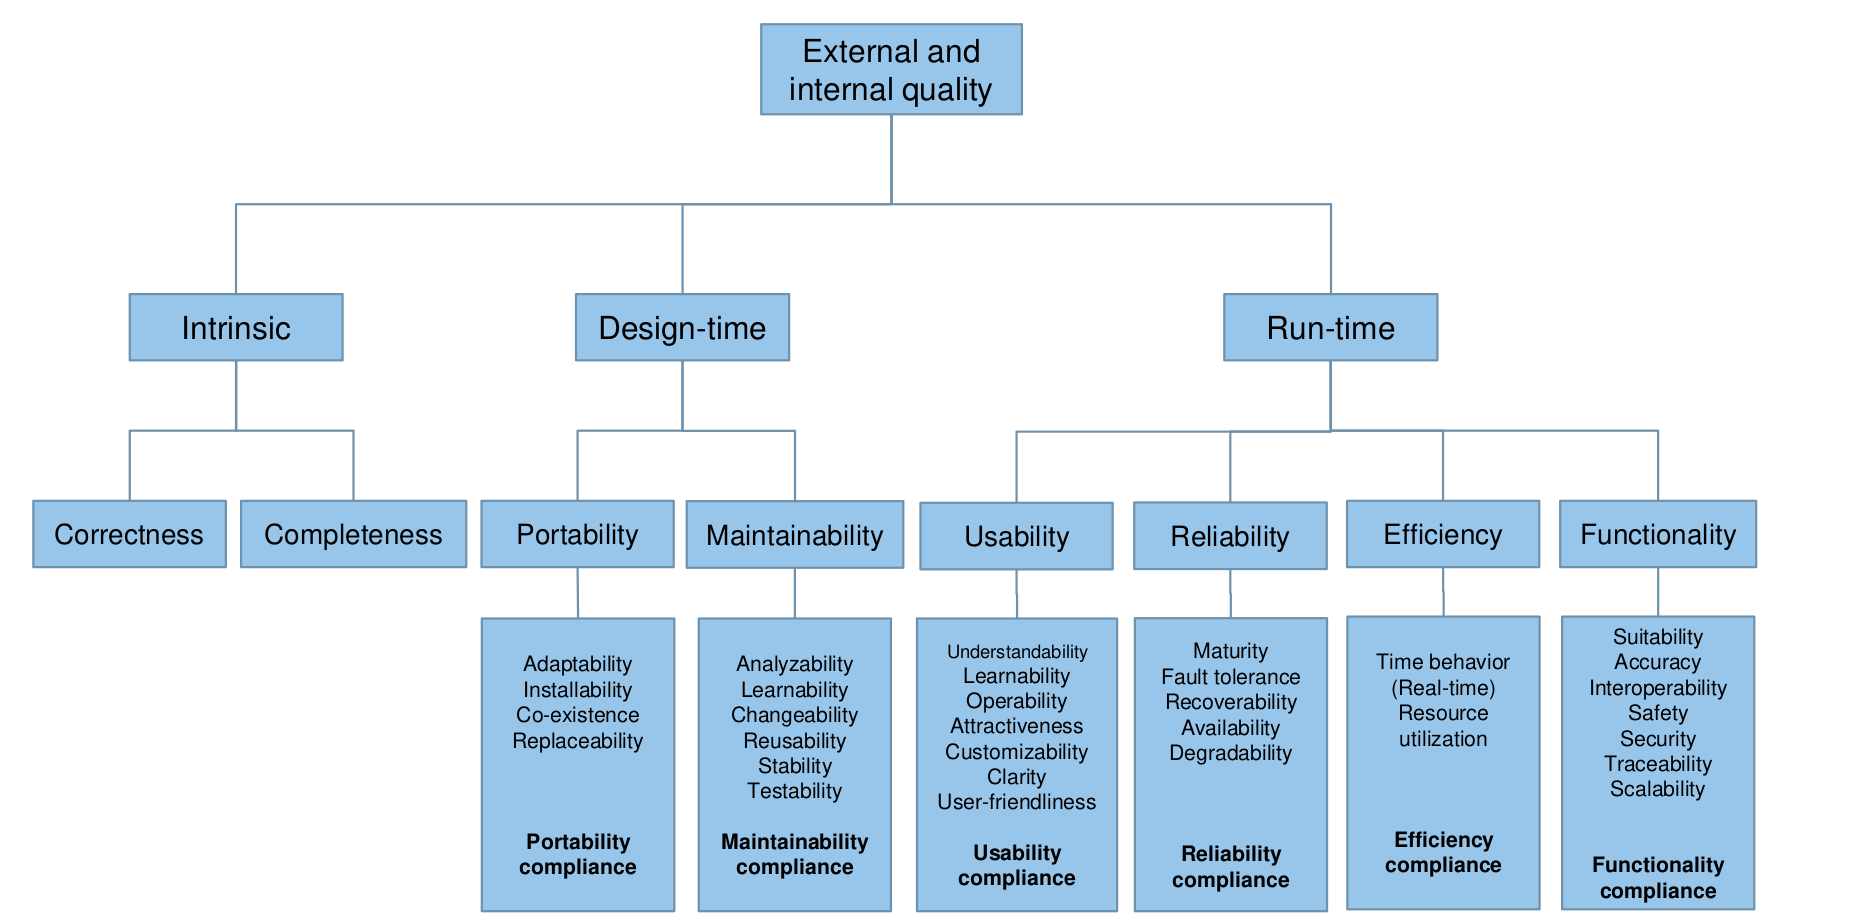
\includegraphics[width=\linewidth]{images/types_of_quality.png}
    \caption{Types of Quality}\label{fig:se_types_of_quality}
\end{figure}
